\subsection{Problematiza\c c\~ao da Revis\~ao} \label{subsec: problematização da revisão}

Nesta subseção, é discutido um problema de pesquisa que pode ser compreendido por diversos leitores. A Figura \ref{fig:serie-temporal} apresenta um mapa conceitual das publicações, destacando a importância dos autores como base para esta revisão. Os modelos propostos por esses autores são fundamentais para abordar o problema em questão, uma vez que a previsão em séries temporais é um desafio de grande significado por si só.

\begin{figure}[H]
	\centering
	\caption{Mapa conceitual do problema de pesquisa}
	\label{fig:serie-temporal}
	\includegraphics[width=0.9\linewidth]{Revisao/Figuras/"Série temporal"}
	
	Fonte: Elaboração própria 
\end{figure}

O mapa conceitual apresentado na Figura \ref{fig:serie-temporal} ilustra a relação entre as palavras-chave que estão relacionadas ao problema em questão, proporcionando uma visão clara do que será abordado ao longo do trabalho. Esse mapa contribui para a identificação dos principais tópicos de pesquisa e das questões que serão exploradas posteriormente.

\begin{enumerate}[start=1, label = {\textbf{Q} \arabic* } ]
	\item \label{questão:rev1}Quais os autores que mais publicam sobre o assunto de séries temporais?
	\item \label{questão:rev2}Quais os países que mais publicam sobre o assunto? 
	\item \label{questão:rev3}Quais as áreas que mais publicam sobre o tema?
	\item \label{questão:rev4}Quais são as obras mais influentes na análise de séries temporais?
\end{enumerate}

\subsection{Metodologia}\label{subsec:met da revisão}

Nesta subseção, é fornecida uma explicação detalhada de como a revisão foi conduzida, abrangendo desde a análise do banco de dados até a conclusão final da revisão. São apresentados os passos e critérios adotados para a seleção dos artigos, bem como os procedimentos utilizados para a extração e análise dos dados. A subseção visa esclarecer de forma clara e objetiva todo o processo metodológico empregado durante a realização da revisão.

\begin{figure}[H]
	\centering
	\caption{Etapas da Revisão.}
	\label{fig:rsl}
	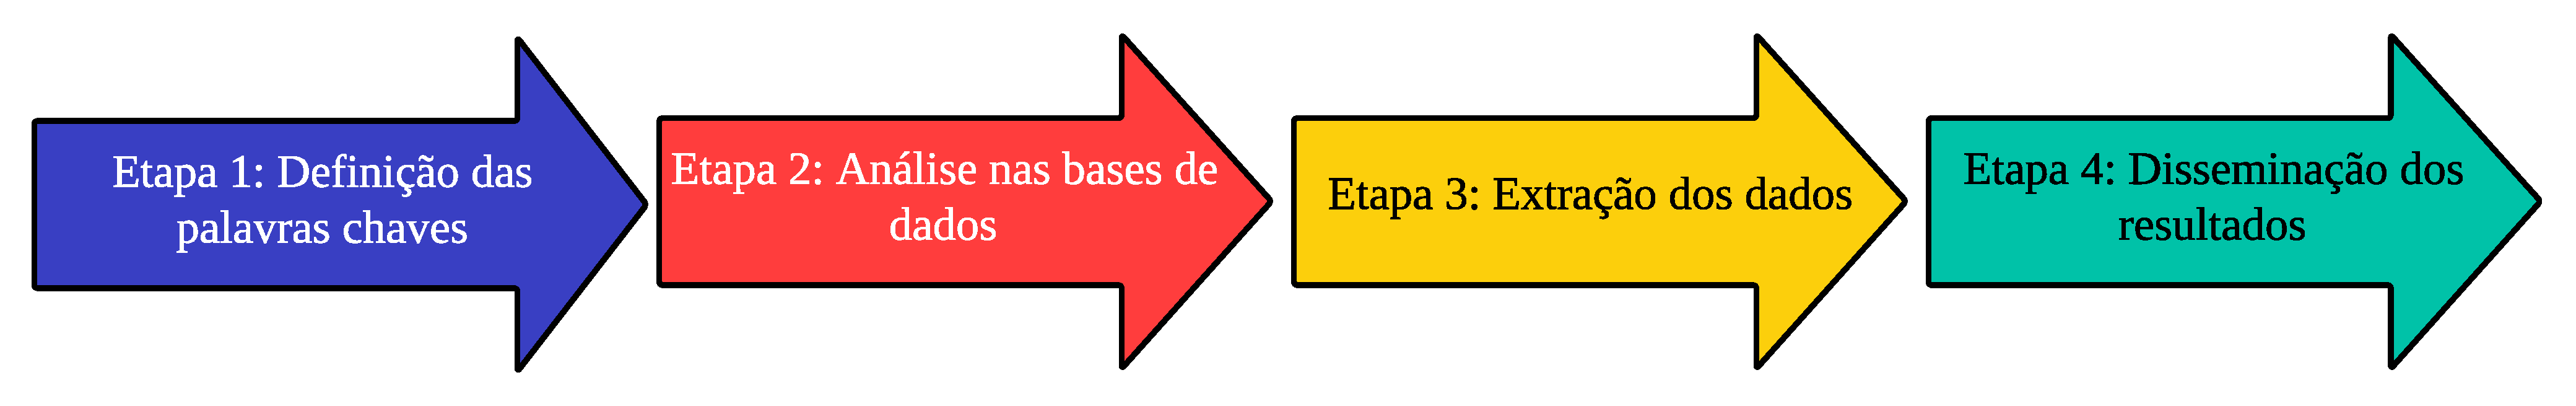
\includegraphics[width=0.9\linewidth]{Revisao/Figuras/RSL}
	
	Fonte: Adaptado de \citeonline{MARTINS201671}
\end{figure}


\begin{enumerate}[start=1, label={\textbf{Etapa} \arabic*}]
	
	\item \label{etp:rev-1} A Figura \ref{fig:rsl} apresenta uma adaptação da metodologia proposta por \citeonline{MARTINS201671} para a realização desta revisão sistemática. Inicialmente, foram realizadas buscas nos bancos de dados Scopus, Web of Science e Lens, selecionando algumas bases relevantes para o tema da pesquisa.
	
	
\textbf{Campo de pesquisa Scopus}

\textbf{\textit{TITLE-ABS-KEY (``time series forecasting")  AND  TITLE-ABS-KEY (``time series analysis")  AND  ( LIMIT-TO ( DOCTYPE ,  ``ar" ) )  AND  ( LIMIT-TO ( LANGUAGE ,  ``English" ) )  AND  ( LIMIT-TO ( PUBYEAR ,  2022 )  OR LIMIT-TO ( PUBYEAR ,  2021 )  OR  LIMIT-TO ( PUBYEAR ,  2020 )  OR  LIMIT-TO ( PUBYEAR ,  2019 )  OR  LIMIT-TO ( PUBYEAR ,  2018 )  OR  LIMIT-TO ( PUBYEAR ,  2017 ) )}}

\textbf{Campo de pesquisa na Web of Science}

\textit{\textbf{``times series forecasting" (All Fields) and ``time series analysis" (All Fields)}} (Publication Years: 2022 or 2021 or 2020 or 2019 or 2018 or 2017) (Document Types: Articles) (Languages: English)

\textbf{Campo de pesquisa de Lens}

\textit{\textbf{Scholarly Works (11) = ( ``time series forecasting" ) AND ( ( ``time series analysis" ) AND ( ``nonlinear forecasting" ) ) }}
Filters: Year Published = ( 2016 - 2022  ) Publication Type = ( journal article  )\\
	
	Para todas as bases de busca, foram considerados os últimos 6 anos, com exceção do Lens, que retornava poucos artigos. Nesta etapa, foram utilizadas palavras-chave que se adequam melhor à pesquisa, como \textit{time series forecasting and time series analysis and nonlinear forecasting}.
	
	\item \label{etp:rev-2} No cruzamento das palavras-chave, obteve-se um número considerável de artigos, sem restringir a área em que cada um pode ser publicado. A Tabela \ref{tb1} apresenta a tabulação dos resultados obtidos, sem excluir duplicatas, que serão tratadas na seção \ref{subesec:resul da revisão}.
	
	\item \label{etp:rev-3} Nesta etapa, é realizada uma avaliação preliminar de cada artigo obtido, sem aplicar nenhum filtro anual nas buscas. Analisar todos os artigos dessa maneira resultaria em um número elevado, por exemplo, no banco de dados Scopus seriam 498 artigos, na Web of Science seriam 140 artigos e no Lens, que retorna poucos artigos, seriam 11 artigos, totalizando 649 artigos sem remover duplicatas. É importante ressaltar que esses artigos passaram apenas pelo filtro de idioma inglês e de serem artigos, visando aprimorar a busca e a tomada de decisões. Ao aplicar o filtro dos últimos 6 anos, obteve-se um número mais gerenciável de artigos para análise. Levando em consideração a diferença entre essa estimativa apresentada na Tabela \ref{tb1} e a quantidade de artigos restantes após a remoção de duplicatas, temos menos de 356 artigos para análise. É válido lembrar que, ao remover as duplicatas, esse número pode diminuir ainda mais, atingindo o objetivo proposto neste trabalho.
	
	\item \label{etp:rev-4} Nesta etapa, é realizada uma análise mais aprofundada do conteúdo dos artigos selecionados, levando em consideração as áreas de especialização e correlação com séries temporais. Como esta revisão está inserida no contexto de um programa de mestrado em Engenharia de Produção e Sistemas, vale a pena analisar a correlação com áreas como Matemática. A Figura \ref{fig:areas} mostra que as áreas mais relevantes para a pesquisa são \textbf{Informática, Engenharia e Matemática}, representando 50\% das publicações. Portanto, a pesquisa está alinhada com a utilização de conceitos matemáticos básicos para realizar uma estimativa do número de artigos que podem ser eliminados. Estima-se que cerca de 481 artigos possam ser excluídos, porém essa estim
	
	ativa não possui uma base sólida. Utilizando o software Mendeley Desktop para obter o número exato de artigos sem duplicatas, chegou-se a um total de 308 artigos.
	
\end{enumerate}